\documentclass{article}

\usepackage[utf8]{inputenc}
\usepackage[T1]{fontenc}
\usepackage{palatino}
\usepackage{graphicx}
\usepackage{fullpage}
\usepackage{float}
\usepackage{hyperref}
\usepackage{arydshln}

\usepackage[parfill]{parskip}
\usepackage[font=small, labelfont=bf]{caption, subcaption}

\title{INFOF-409 --- Learning Dynamics\\ Assignment 2 --- Evolutionary Game Theory}
\author{Robin Petit\\ MA1-CS -- ULB}
\date{November 23, 2017}

\begin{document}

\pagenumbering{Roman}
\maketitle
\tableofcontents
\newpage
\pagenumbering{arabic}
\setcounter{page}{1}

\section{Part I}

Figure~\ref{fig:coop proportion} shows the cooperation proportion for different grid (lattice) sizes,
for different neighbourhood types, and for different payoffs. In this first part, only the first two
subfigures are of interest: the upper left one presents the proportion of cooperation level for
different lattice sizes $n \times n$ (respectively $n=4,8,12,20,50,100,500$) when playing Prisoner
Dilemma with best neighbour replication rule and with Moore neighbourhood, and the upper right one
is the same configuration bu with Von Neumann neighbourhood instead.

\begin{figure}[!b]
\hspace{-2.5cm}
\vspace{-.7cm}
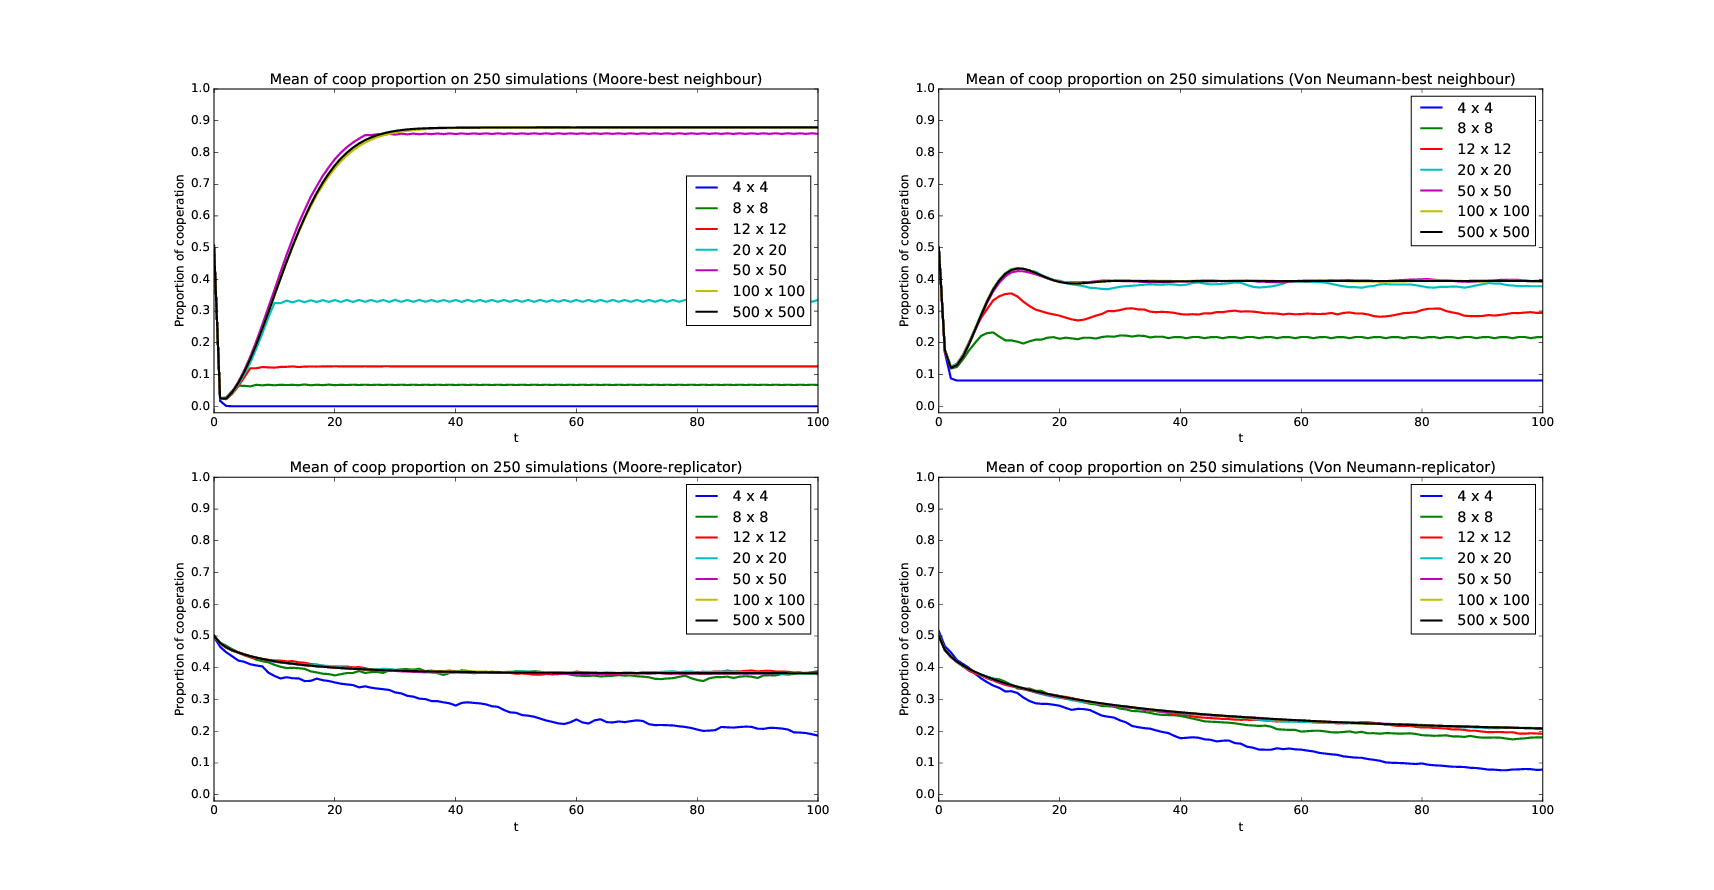
\includegraphics[width=1.3\textwidth]{imgs/means-250.png}
\caption{Proportion of cooperation level according to lattice size, neighbourhood size, and replication
rule (coupled with payoff matrix) on 250 evolution steps. First plot represents the cooperation
proportion of square lattice (in the sense of square dimension: $n \times n$ since lattices are
considered as placed on the surface of a torus) playing weak Prisoner Dilemma with Best Neighbour
replication rule and Moore neighbourhood. Second plot is the same as the first one with Von Neumann
neighbourhood instead of Moore neighbourhood. Third plot represents the cooperation proportion of
square lattices playing Snowdrift Game with stochastic replication rule and Moore neighbourhood.
Finally, the last plot is the same as the third one with Von Neumann neighbourhood instead of Moore
neighbourhood.
\label{fig:coop proportion}}
\end{figure}

\subsection{Moore Neighbourhood Analysis}

\subsubsection{Cooperation Level}

What one can see is that, first of all, with Moore neighbourhood, the larger the lattice, the higher the
cooperation level is in the lattice. A hypothesis that one could express is that for small lattices
such as 8~x~8 or 12~x~12, the lattice reaches some sort of steady state very quickly since there is
not much distance overall that would allow more complex patterns to emerge.

Also, we see that for a 4x4 lattice, the cooperative players tend to vanish in only two periods.
This is due to the fact that in such a small space, there cannot be enough of cooperative players
clustered together, which would allow them to increase their individual payoff, they are surrounded
by too many defecting players. Therefore, in a 4~x~4 lattice with Moore neighbourhood, the cooperation
is not viable.

Another interesting observation is that even though instructions required to test lattice sizes up to
50~x~50, when plotting the mean  cooperation level for lattices even bigger (e.g. 100~x~100 and 500~x~500),
we observe that the cooperation level asymptotes to around $88\%$. A possible interpretation is that
as the lattice is sufficiently large, cooperative players have the possibility to expand on the lattice,
but will not cover it entirely because a defecting player still have an advantage over cooperative players
in some circumstances. For instance, a defecting player surrounded by cooperative players will have a
payoff of 56. Then, if one of its cooperative neighbours has less than six cooperative neighbours,
his payoff will be lower or equal to 50. In this situation, it is clear that the defecting method is
preferable. Also, the high level of cooperation at \textit{stability} can be explained by this same
interpretation: in a large lattice, the majority tends to cooperate, but defecting only represents an
advantage for a player with many cooperative neighbours. Therefore, a small portion defects, but this
proportion cannot be too big otherwise defecting stops being an advantage.

We can also observe that at time $t=1$, the cooperation level of the lattice crashes down to around
$2\%$. The explanation only requires the update method, and no the neighbourhood type, which is why
we will make the same observation with Von Neumann neighbourhood. In this first part, the update
method is \textit{Best neighbour}, meaning that at each period, every player (agent) will change its
action by replacing it by the action of its neighbour having the best payoff (if this payoff is
bigger than their own payoff, otherwise they don't change action). Also, the lattice is initialized
randomly with a $50\%$ proportion of cooperative players and $50\%$ of defecting players. Therefore,
one can assume that in average (more and more reasonable assumption as the lattice size increases)
the cooperative and defecting players are scatter along the lattice, and not clumped together. This
reduces highly cooperative players' payoff, and then makes cooperative players change to defecting
for next period, whereas in general defecting players' wouldn't change to cooperation since their
payoff is bigger.

Yet, despite all of the differences in behaviour according to the lattice size, all curves on the first
subplot all share one property: in average, they all converge to a stable cooperation proportion, and
the time required to reach this stability seems to be dependent on the value of the equilibrium.
This can be explained by the sudden drop that we observe at first step: the cooperation level on the
lattice crashes down, and then has to climb up to the stable point. So, the higher the stability, the
longer the lattice must \textit{wait} to reach that stability.

\subsubsection{Spatial Representation}

\begin{figure}[!b]
	\begin{subfigure}{\textwidth}
		\hspace{-2.5cm}
		\vspace{-.5cm}
		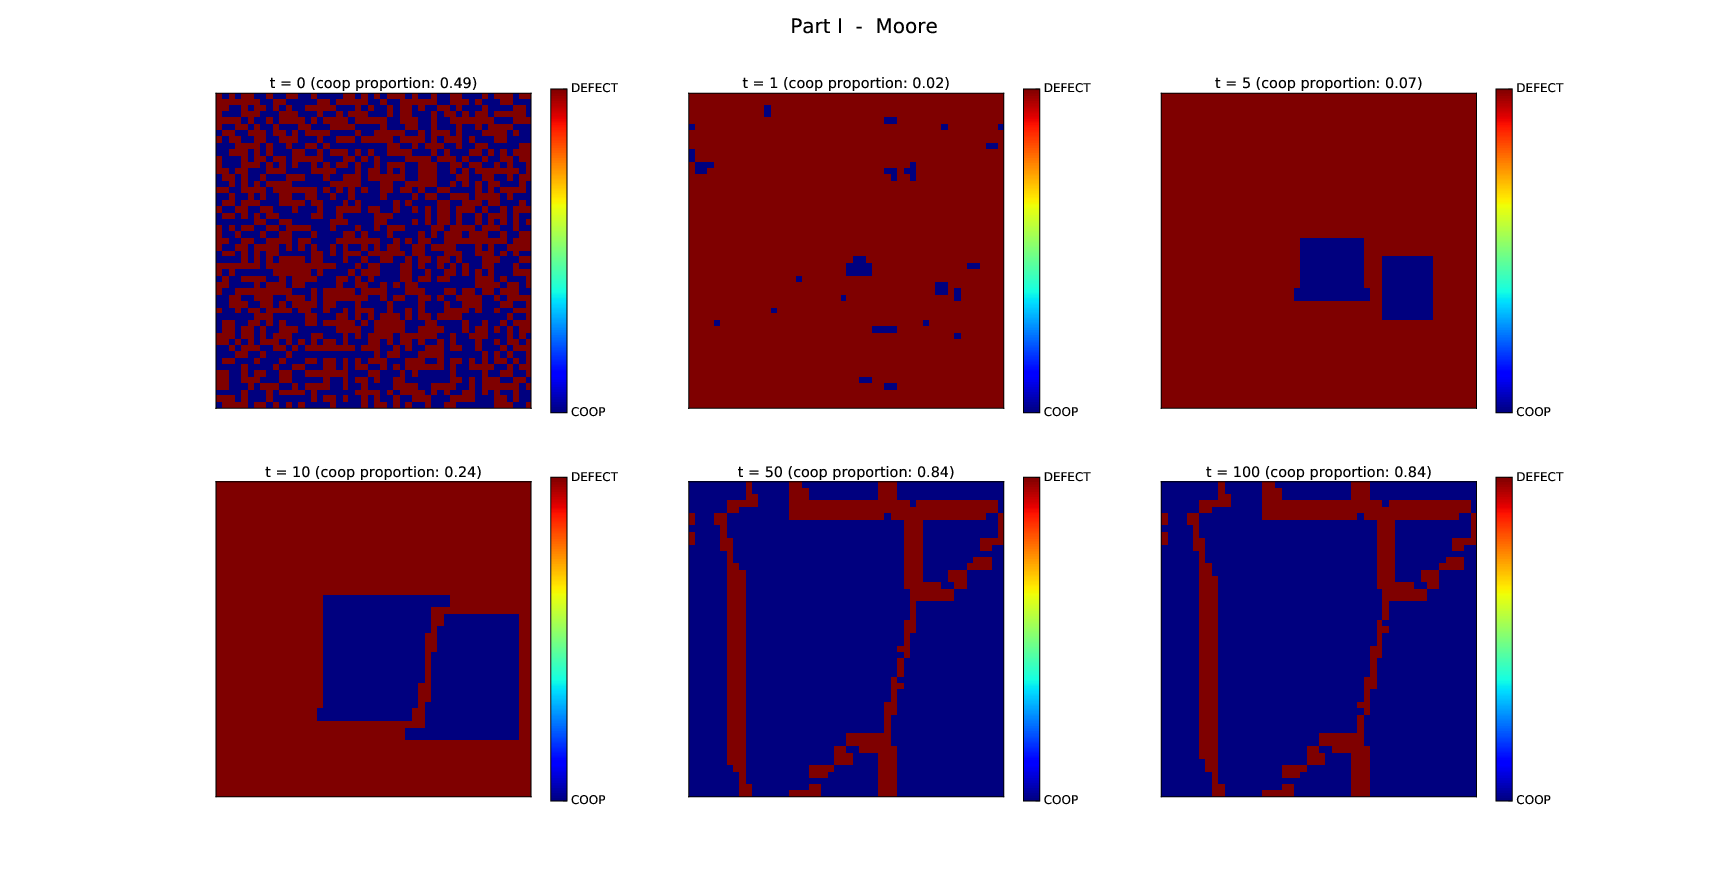
\includegraphics[width=1.25\textwidth]{imgs/part1_Moore_periods.png}
		\subcaption{Spatial view of the lattice at different periods.\label{fig:2a}}
	\end{subfigure}
	\begin{subfigure}{\textwidth}
		\centering
		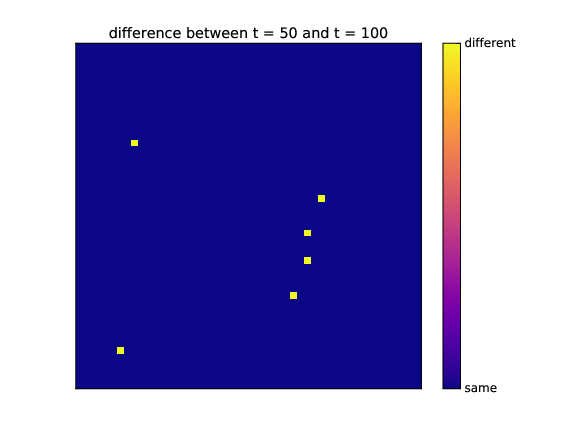
\includegraphics[width=.4\textwidth]{imgs/part1_Moore_periods_difference.png}
		\subcaption{Difference of actions in lattice between periods 50 and 100.\label{fig:2b}}
	\end{subfigure}
	\caption{Spatial representation of Part I with Moore neighbourhood\label{fig:Spatial Representation Part I Moore}}
\end{figure}

Figure~\ref{fig:Spatial Representation Part I Moore} shows the spatial representation of the lattice at
times $t = 0, 1, 5, 10, 50, 100$. On Figure~\ref{fig:2a}, we see that at $t=0$, the players are scattered
randomly, and that at $t=1$, the cooperative players proportion suddenly drops to $2\%$, and then
increase slowly to $84\%$.

We can see that at time $t=1$, there are only a few cooperative players left and that, in the most
part have less than 4 cooperative neighbours. By the discussion above, this leads them to change action
to defection. At time $t=5$, we see clearly that only two blocks of cooperative players were big enough
to not change to defection, and to expand. At time $t=10$, we can see that these blocks are the same,
but have just expanded (meaning that their payoff was sufficiently big to force defecting neighbours
become cooperative).

Still at $t=10$, we observe a clear boundary of defecting players between the two observable blocks
of cooperative players. This phenomenon is explained above in the discussion on the convergence
of cooperation level. For the defecting players in this region, they have between 3 and 6 cooperative
neighbours, leading to a high payoff.

These boundaries take the form of \textit{strips} of defecting players between cooperative players,
and can be observed even further with $t > 10$: for $t=50$ and $t=100$.

Also, even though the lattice looks identical between times $t=50$ and $t=100$, it has actually changed,
but very slightly, which is shown in Figure~\ref{fig:2b}. We can interpret this as stability, especially
when looking at the difference in Figure~\ref{fig:2b}: only 6 players have changed action. Note that
more can have changed their action between these two periods, but in this case, they need to have settled
back to their action of time $t=50$. Therefore, the behaviour can either be complete stability: players
don't change actions anymore, or periodicity.

What can be concluded from this analysis is that in the configuration of the first part, with a Moore
neighbourhood, a cooperative strategy is not viable if the amount of defecting neighbours is too high,
but if enough cooperative players are clumped together in a region of space, then they will \textit{convert}
their defecting neighbours since their payoff will be high enough.

\subsection{Von Neumann Neighbourhood Analysis}

\subsubsection{Cooperation Level}

Looking back at Figure~\ref{fig:coop proportion}, on the second subplot we can see that a lot of observations
made in the previous subsection still hold: there is a sudden drop in the cooperation level at time
$t=1$; the larger the lattice, the higher the steady value; the higher the steady value, the more time
is required to reach \textit{stability}. Note that "stability" is written in italic because the so called
\textit{stability} studied here is an average pseudo-stability: an individual lattice situation could
either completely miss the equilibrium we are discussing, or miss any equilibrium by having seemingly
chaotic behaviour. Yet, when considering the behaviour as an average of many different lattices, it may
be considered stable.

Despite sharing many common features with the first study case, this second one has a few differences.
First of all, we can see that there is a lot less variance in the stability values reached by the different
lattice sizes: grids smaller than 20~x~20 have a higher average cooperation level stability than in the
previous study, and grids bigger than 20~x~20 have a smaller average cooperation level stability than
in the previous case. The 20~x~20 lattice also increased a bit.

But not only are these values closer to one another, we especially observe that the asymptote value is
more than halved. We can hypothesize that as neighbourhood is reduced compared to previous case, cooperative
players have a harder time \textit{spreading} their strategy since only fewer defecting neighbours may
change their strategy to cooperation.

Also, we can see that on the 4~x~4 lattice, cooperation doesn't die out as it did with Moore neighbourhood.
This could either be due to the averaging of 250 simulations or be a general persistence of cooperative
players. It seems reasonable to consider this to not be due to the averaging: in a Von Neumann neighbourhood,
it is viable for a cooperative player to have a single cooperative neighbour, whereas it is not in a
Moore neighbourhood.

\begin{table}[!h]
\vspace{.5cm}
\begin{subtable}{.3\textwidth}
\centering
\begin{tabular}{:c|c|c|c:}
\hdashline
D & D & D & D \\ \hline
D & D & \textbf{C} & \textbf{C} \\ \hline
D & D & D & D \\ \hline
D & D & D & D \\ \hdashline
\end{tabular}
\caption{Action of each player on the lattice}
\end{subtable}\hspace{.025\textwidth}%
\begin{subtable}{.35\textwidth}
\centering
\begin{tabular}{:c|c|c|c:}
\hdashline
0 & 0 & 7 & 7 \\ \hline
7 & 7 & \textbf{10} & \textbf{10} \\ \hline
0 & 0 & 7 & 7 \\ \hline
0 & 0 & 0 & 0 \\ \hdashline
\end{tabular}
\caption{Payoff of each player on the lattice for Von Neumann neighbourhood}
\end{subtable}\hspace{.025\textwidth}%
\begin{subtable}{.3\textwidth}
\centering
\begin{tabular}{:c|c|c|c:}
\hdashline
7 & 7 & 14 & 14 \\ \hline
7 & 7 & \textbf{10} & \textbf{10} \\ \hline
7 & 7 & 14 & 14 \\ \hline
0 & 0 & 0 & 0 \\ \hdashline
\end{tabular}
\caption{Payoff of each player on the lattice for Moore neighbourhood}
\end{subtable}

\caption{Example of situation on a 4~x~4 lattice where only two cooperative players is viable (stable) with
Von Neumann neighbourhood but is not with Moore neighbourhood. Cooperative players are marked in boldface
to make them easier to locate.
Borders are marked in dashed lines only to emphasize the torus topology of the lattice: \textit{borders} are
\textbf{not} borders but the lattice wraps back on itself.
\label{tab:viable situation VN}}
\end{table}

As can be seen in Table~\ref{tab:viable situation VN}, it is possible to find a non-decreasing situation
(in the sense of the cooperation level) with only two cooperative players on a 4~x~4 lattice with a Von
Neumann neighbourhood. This is impossible with a Moore neighbourhood. The smallest non-decreasing situation
on a 4~x~4 lattice with Moore neighbourhood contains 4 cooperative players arranged as follows: one placed
arbitrarily and the three others placed in its Von Neumann neighbourhood (i.e. non diagonal neighbours).
This is due to the fact that Von Neumann neighbourhood forces two neighbours to have an empty common
neighbourhood, whereas Moore neighbourhood forces two neighbours to have exactly a common neighbourhood
of length 4.

Note that as the lattice borders are identified by parallel pairs, i.e. as the lattice is a torus, modulo
rotations, this situation is the only one possible.

One last thing to note is that after the sudden drop in the cooperation proportion, this cooperation level
reaches a local maximum and decreases slightly afterwards. This is easy to see for grids 20~x~20 and bigger.
This phenomenon may be perceived for 8~x~8 and 12~x~12 but is very tiny, and the curves are less smooth,
so it is to interpret with care.

This double-bump effect is hard to interpret because it appears on the averaged plot. Therefore, it would
be needed to explore many lattices individually to see if this phenomenon appears every time, or if it is
due to the averaging of several different behaviours.

\subsubsection{Spatial Representation}

Figure~\ref{fig:Spatial Representation Part I VN} shows the spatial representation of the 50~x~50 lattice
at times $t=0,1,5,10,50,100$. The first thing to note is that at time $t=1$, the cooperative players have
heavily dropped (reduced to around a third than the cooperation level at time $t=0$) just like before,
but the magnitude of the phenomenon is completely different: divided by 25 for Moore neighbourhood and
by 3 for Von Neumann neighbourhood. This can also be seen in Figure~\ref{fig:coop proportion}: the drop
is not as strong on the second plot, and also it takes longer to fully drop. With Moore neighbourhood,
there is a sudden drop at time $t=1$, and the proportion level stays approximately constant at time $t=2$
(an equal amount switches from cooperation to defection than from defection to cooperation) whereas
with Von Neumann neighbourhood, the drop takes two step to reach around $12\%$.

Compared to Figure~\ref{fig:2a}, we clearly see that in this case, even though cooperative players get
scattered along the lattice, small clusters still remain whereas in first study, cooperative players only
remained in quite large blocks (at least large enough to have a high enough payoff).

In the end, we see that the amount of cooperative players is lower than in Figure~\ref{fig:2a}, as expected
by looking at Figure~\ref{fig:coop proportion}, and also that defecting players don't form strips as before
but form somehow large clusters, probably because cooperative players aren't able to break through the
defecting borders.

We can also observe that at time $t=10$, the cooperative players seem to form diamond shapes versus rectangles
in Figure~\ref{fig:2a}, which is quite clear due to the neighbourhood shape, and then due to the propagation
vectors.

In comparison with Figure~\ref{fig:2b}, Figure~\ref{fig:3b} shows that the lattice is way less stable in this
second study case than in the first one: even though the proportion of cooperative players stays roughly
constant, the lattice itself is not static at all.

\begin{figure}%[!h]
		\begin{subfigure}{\textwidth}
		\hspace{-2.5cm}
		\vspace{-.5cm}
		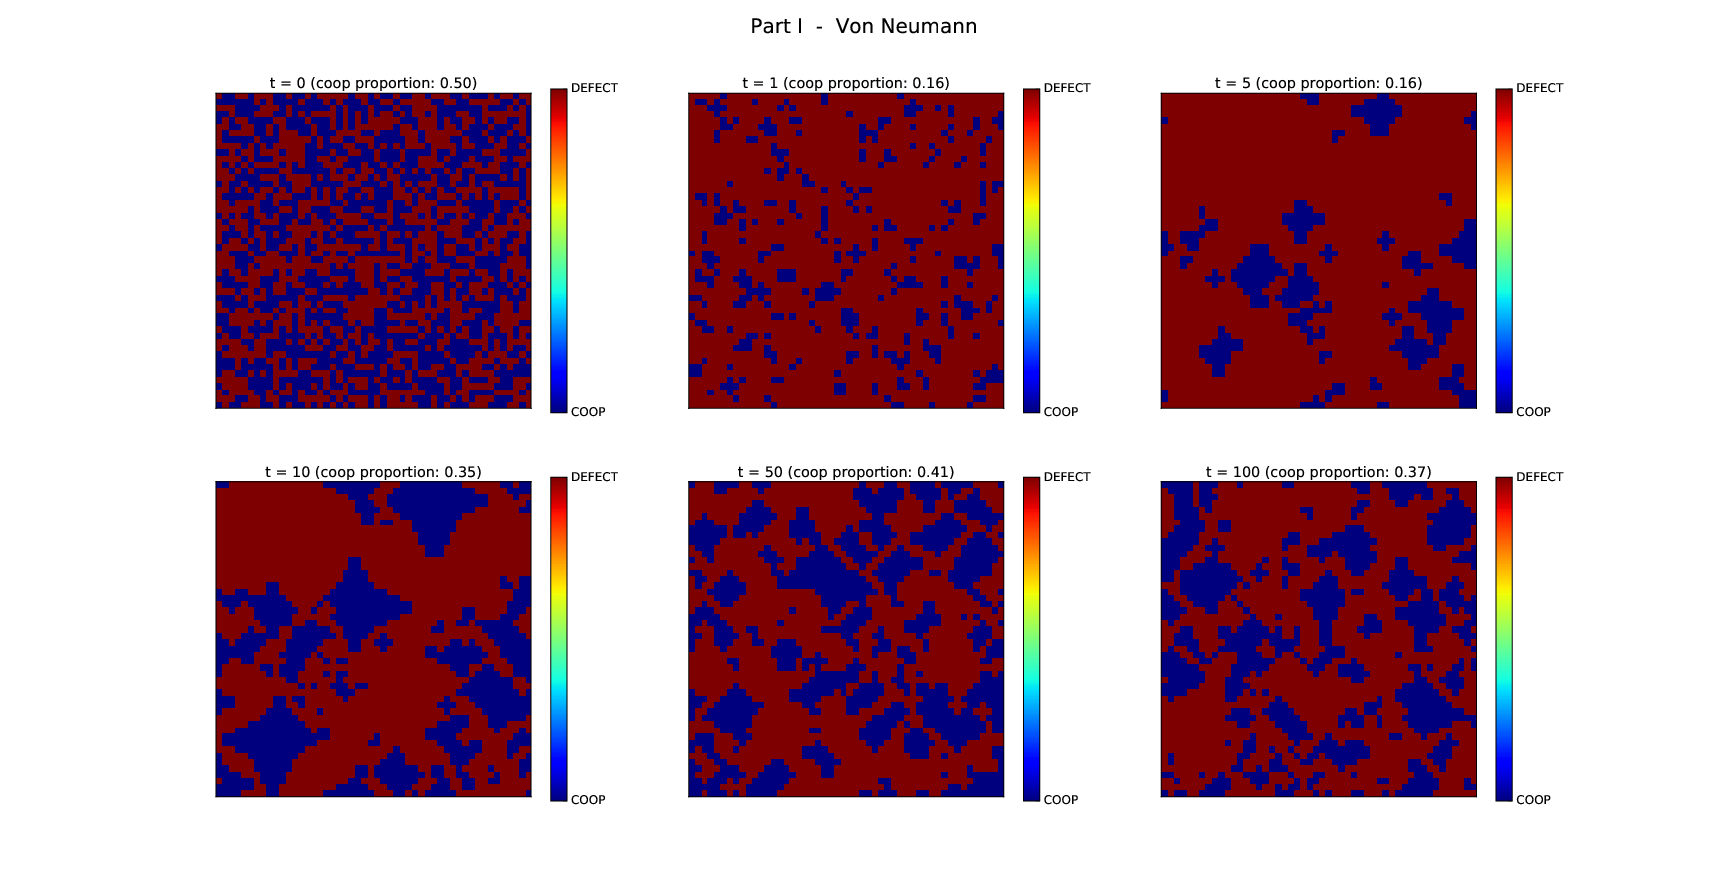
\includegraphics[width=1.25\textwidth]{imgs/part1_VN_periods.png}
		\subcaption{Spatial view of the lattice at different periods.\label{fig:3a}}
	\end{subfigure}
	\begin{subfigure}{\textwidth}
		\centering
		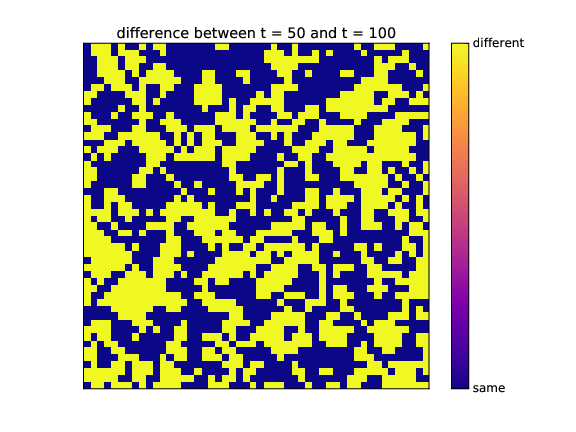
\includegraphics[width=.4\textwidth]{imgs/part1_VN_periods_difference.png}
		\subcaption{Difference of actions in lattice between periods 50 and 100.\label{fig:3b}}
	\end{subfigure}
	\caption{Spatial representation of Part I with Von Neumann neighbourhood.\label{fig:Spatial Representation Part I VN}}
\end{figure}

\newpage

\section{Part II}

In this second part, the update method has changed: for each player, one of the neighbours is chosen randomly
among all of the 8 if Moore, 4 if Von Neumann neighbours, and the player's action is changed to the neighbour's
action with probability $p_{ij} = 1/2 + \frac {W_j-W_i}{2 \cdot 10N}$ where $N$ is the number of neighbours,
$j$ represents the randomly chosen neighbour and $i$ represents the player. The $10$ in the denominator comes from
the difference between $T=10$ and $P=0$, respectively the highest and the lowest payoffs.

This value $p_{ij}$ is indeed a probability because it is between between $0$ and $1$. It is easy to see
that the smallest possible value is when $W_j$ is null, and when $W_i$ is as high as possible, which occurs
if the player $i$ has a payoff of 10 against each of the $N$ neighbours, leading to a payoff of $10N$.
In this case, $p_{ij} = .5 + \frac {-10N}{20N} = .5 - .5 = 0$. Similarly, by setting player $i$'s payoff to 0,
and player $j$'s payoff to be maximal, the probability becomes $p_{ij} = .5 + .5 = 1$.

This probability is then well defined. This formula makes sense to be used because it is linear in the difference
of payoff. Therefore, the higher the neighbour's payoff relative to the player's payoff, the higher the
probability to change the player's action. On the other hand, the higher the player's payoff relative to the
neighbour's payoff, the smaller probability to change. Also, if both the player and its neighbour have the same
payoff, the probability to change is a half, thus allowing to explore more possible patterns in the lattice.

Note that allowing a player to change its action to the action of a neighbour having a lower payoff allows
to explore a broader portion of the state space, reducing the chances of converging, but reducing the chances
of finding a local maximum (considering that the proportion of cooperating players is a value to maximize for
instance).

A possible improvement to the analysis, which will not be performed in this document would be to keep this
probability $p_{ij}$ of changing the action, but changing the way of picking the neighbour. Instead of having
a uniform distribution over the neighbours, one could think of a distribution giving more probability mass
to the neighbours having a high payoff. This leads to a very wide class of possible distributions where
many distributions could be tested. For instance, the probability of picking the neighbour $j$ would be
$W_j/W$, for $W$ the sum of the payoffs of each neighbour (and a uniform distribution if all neighbours
have payoff 0). This method would lead to a uniform distribution with probability $1/N$ for each neighbour
in the situation where all neighbours have the same payoff but could lead to a totally different behaviour
when the neighbours have different payoffs.

For example, considering a Moore neighbourhood with a player having 7 neighbours with a null payoff, and
one with a strictly positive payoff. If the distribution over neighbours is uniform, the player has
probability $7/8 = 87.5\%$ to pick a neighbour with null payoff, whereas with the possible formula
provided above only the neighbour with non null payoff would be selected.

\subsection{Moore Neighbourhood Analysis}

\subsubsection{Cooperation Level}

This subsubsection concerns the third plot of Figure~\ref{fig:coop proportion}.

There are several major differences between this situation and the previous ones. Let's focus the analysis
on the difference between this situation and its homologue of Part I for now. First of all, we can observe
that the cooperation proportion is clearly decreasing with time. A hypothesis would be to say that cooperative
players have a higher probability to change to defect than defecting players have to change to cooperation.

\begin{figure}[!h]
\hspace{-1.8cm}
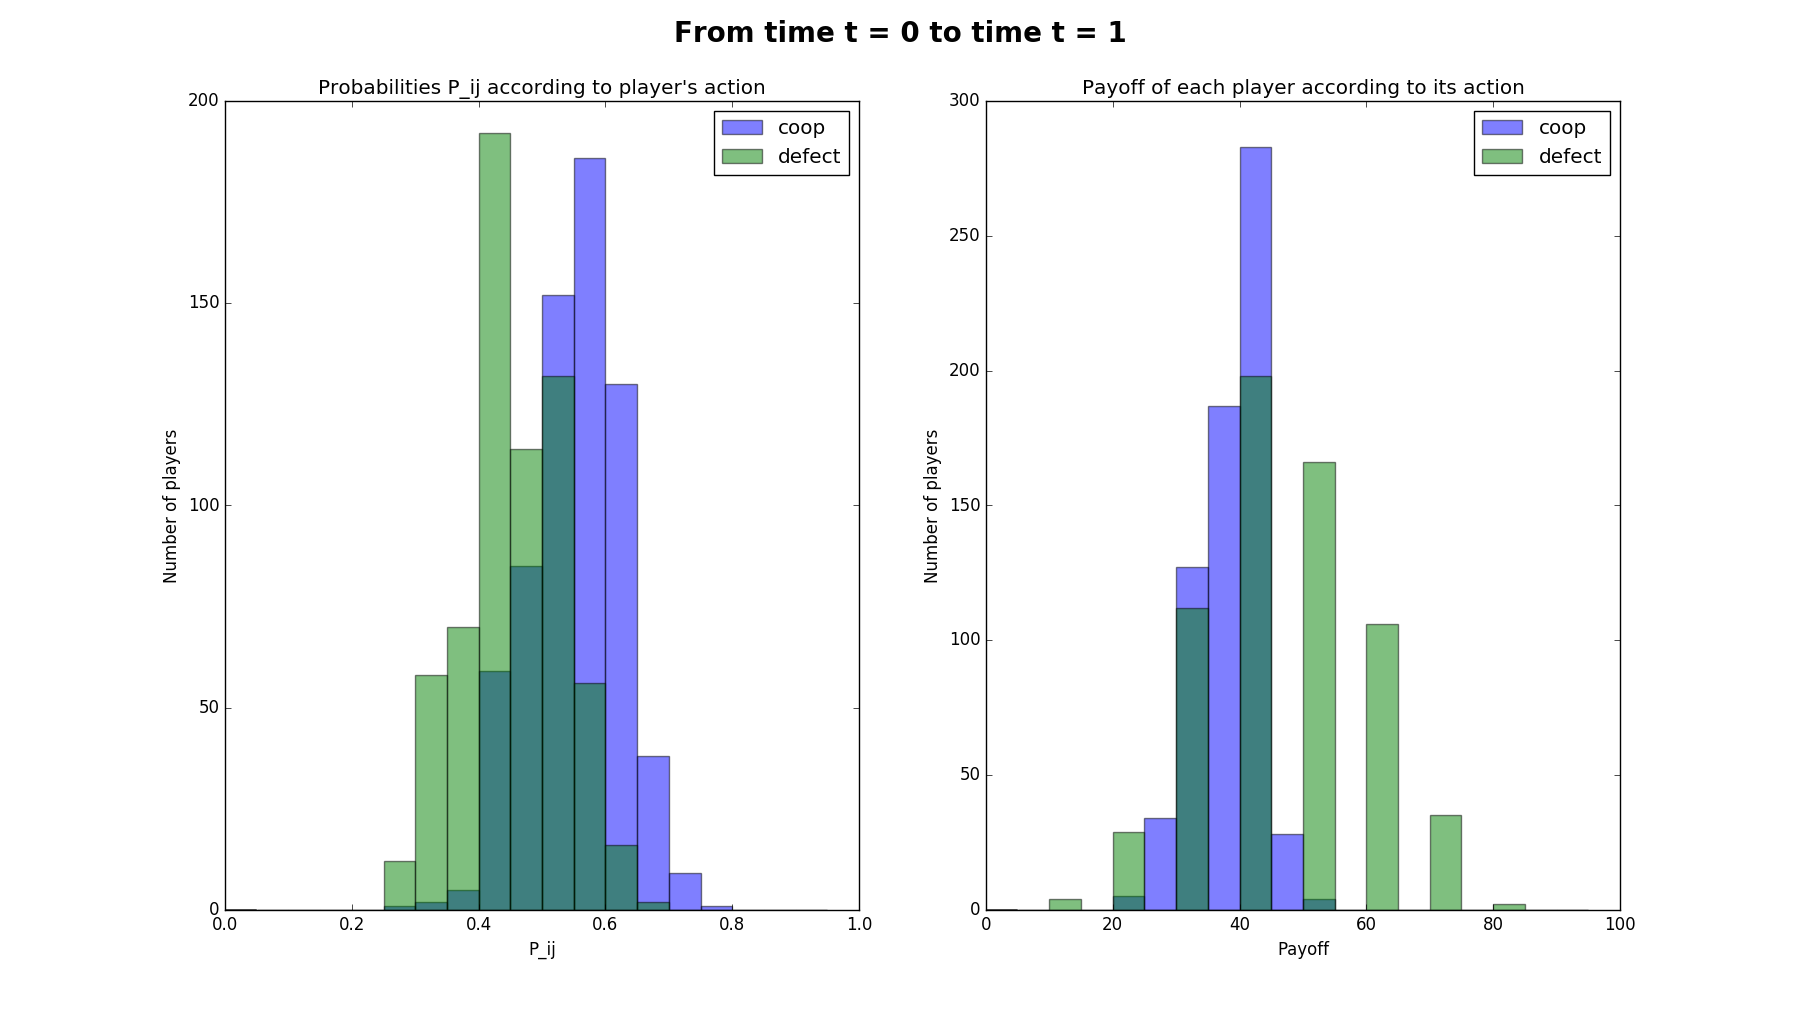
\includegraphics[width=1.2\textwidth]{imgs/part2_diff_coop_defect_0_to_1.png}
\vspace{-1cm}
\caption{Payoff and probability to change action for players on a 50~x~50 lattice at time $t=0$. Every
player considered in the first histogram had either cooperating or defecting strategy, and had picked a
neighbour at random with the opposite strategy; players with a $100\%$ chance of keeping their strategy
were not included. Second histogram represents the payoff distribution of these same players, still
separated by their strategy. \label{fig:Part II hists coop/defect Moore 0 to 1}}
\end{figure}

This hypothesis seems confirmed by Figure~\ref{fig:Part II hists coop/defect Moore 0 to 1} which shows a
significant difference between the probability distribution of changing from cooperation to defection and
from defection to cooperation. Such a difference must have to do with the initial random attribution of
strategies on the lattice, and with the random choice that is performed.

Therefore, the cooperation level decreases with time until these probabilities reach an equilibrium. This
can be observed in Figure~\ref{fig:Part II hists coop/defect Moore 99 to 100}: distribution of probabilities
$p_{ij}$ don't significantly differ anymore between times $t=99$ and $t=100$. This means that the expected
amount of players changing from defection to cooperation is around the same as the number of players changing
from cooperation to defection, thus leading to a stable cooperation proportion.

\begin{figure}[!h]
\hspace{-1.8cm}
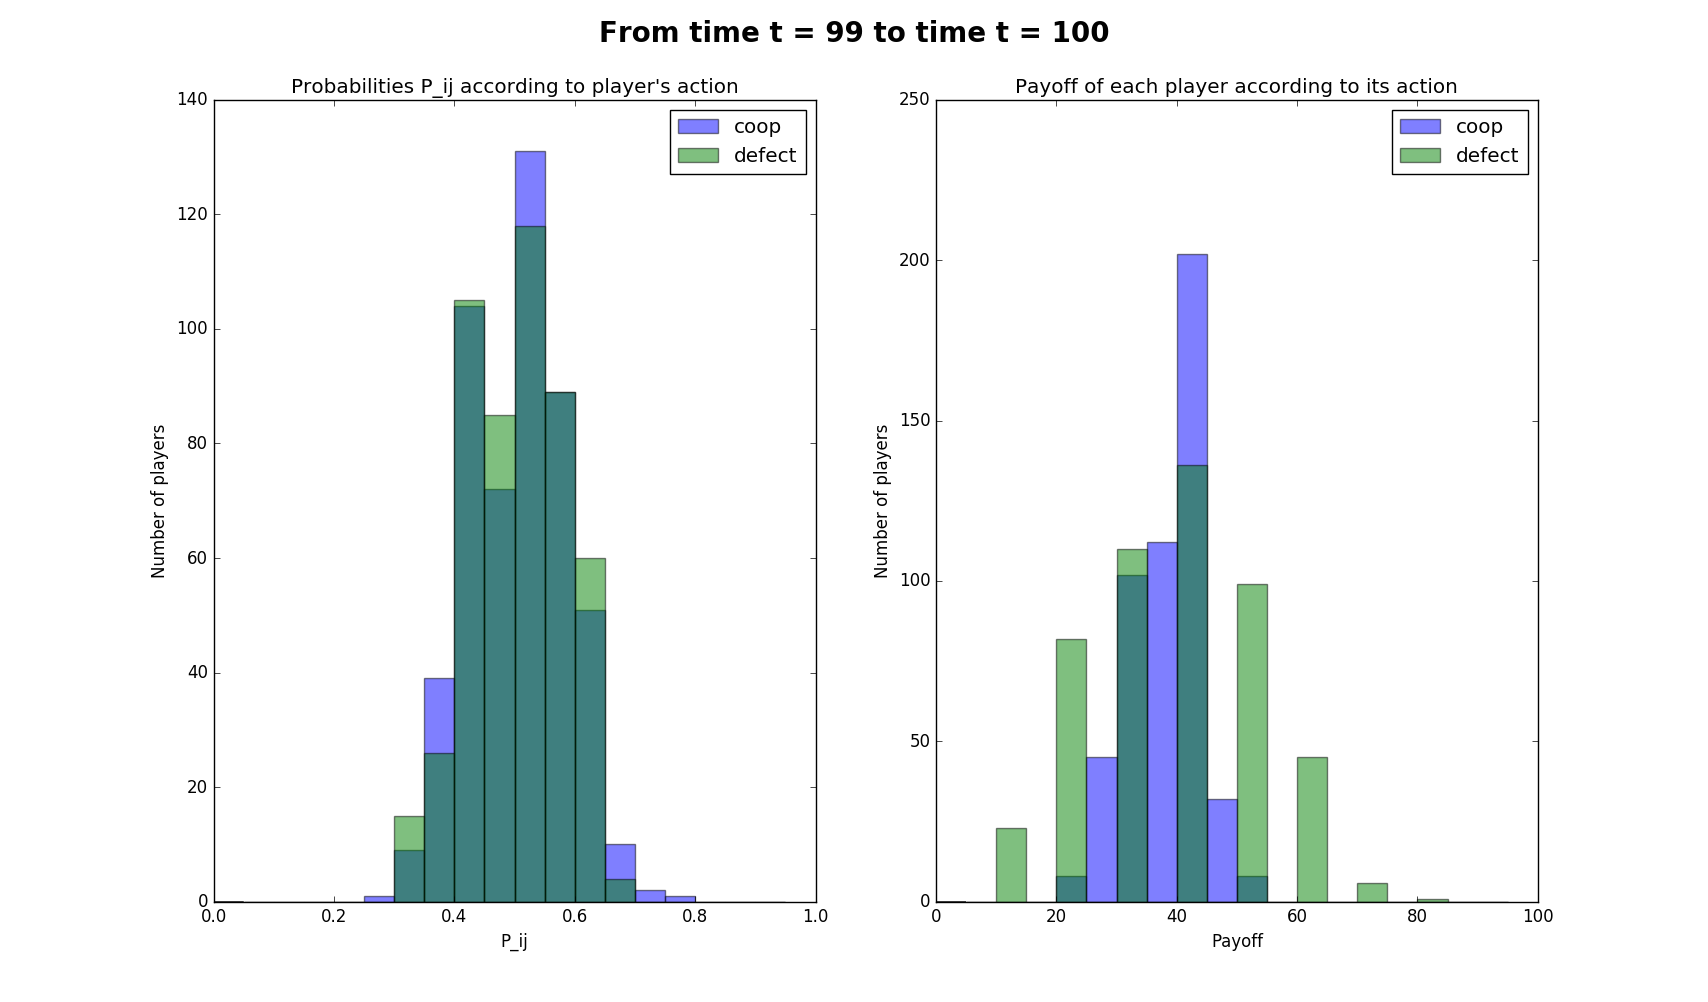
\includegraphics[width=1.2\textwidth]{imgs/part2_diff_coop_defect_99_to_100.png}
\vspace{-1cm}
\caption{Adaptation of Figure~\ref{fig:Part II hists coop/defect Moore 0 to 1} at time $t=99$.
\label{fig:Part II hists coop/defect Moore 99 to 100}}
\end{figure}

As a second major observation, the average cooperation level doesn't depend on the lattice size (except
for the 4~x~4 lattice which will be discussed right after): from 8~x~8 up to 500~x~500, at a given time $t$,
the cooperation proportion is the same. In order to explain this result, we can assume that the discussion
above applies to any lattice size, it only depends on the direct neighbourhood. Also, as opposed to the
first analysis, the fact that a neighbour is chosen at random and that it's not always the best one can
explain why the cooperation level is smaller than in first part: for the cooperating strategy to expand,
a high concentration of cooperative players must be encountered, which has a very lower probability to
appear with the stochastic replicator rule than with the best neighbour replicator rule.

About the 4~x~4 lattice, there are only $2^{16} = 2^{4 \times 4} = 65\,536$ different configurations possible,
thus it is possible to test them all by enumeration, which is not really feasible for a 50~x~50 lattice
since there are $\left(\frac {50}4\right)^2$ more orders of magnitude:
\[\log_{10}\left(2^{50^2}\right) = \log_{10}\left(\left(2^{4^2}\right)^{\left(\frac {50}4\right)^2}\right)
= \left(\frac {50}4\right)^2\log_{10}\left(2^{4^2}\right).\]

By enumerating them all, and by enumerating all the action changes possible in each player's neighbourhood
and plotting the same histogram as in Figures~\ref{fig:Part II hists coop/defect Moore 0 to 1} and
\ref{fig:Part II hists coop/defect Moore 99 to 100}, we obtain what is shown in
Figure~\ref{fig:Part II hists coop/defect Moore all 4x4}: a lower expected probability to update from
defection to cooperation than to update from cooperation to defection. This can explain why 4~x~4 lattices
don't follow the tendency of the other lattices.

\begin{figure}[!t]
\hspace{-1.8cm}
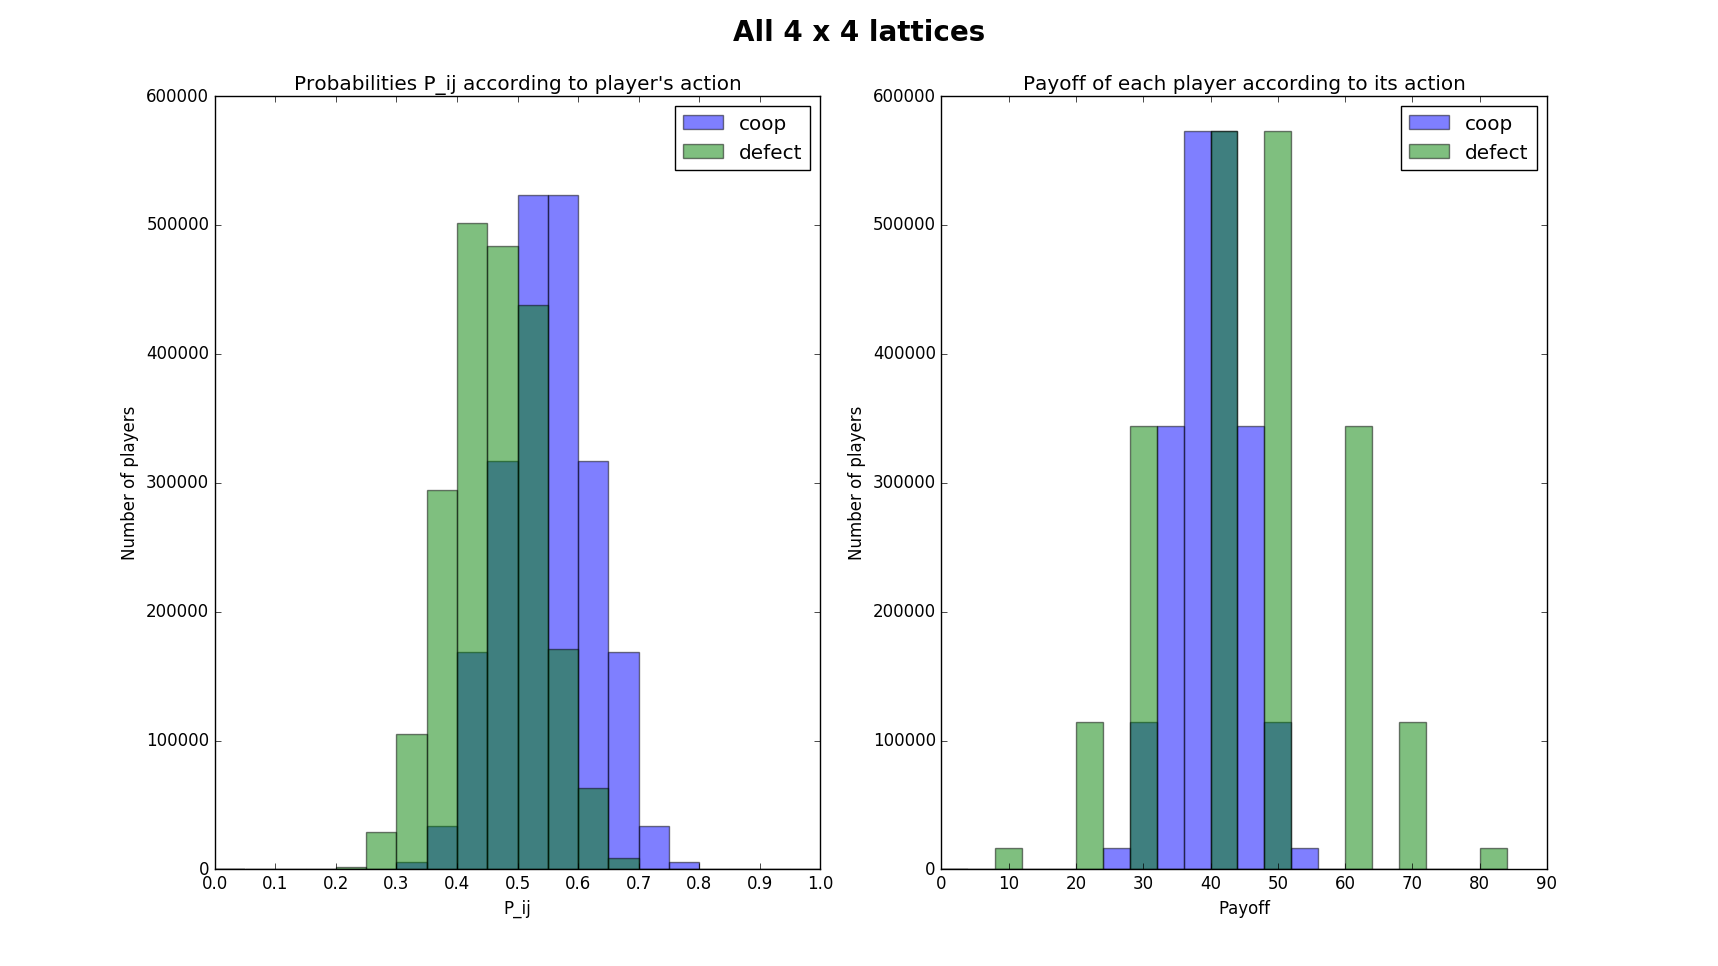
\includegraphics[width=1.2\textwidth]{imgs/part2_diff_coop_defect_0_to_1_4x4.png}
\vspace{-1cm}
\caption{Distribution of the probability $p_{ij}$ and of the payoff of each player according to the action,
computed on all of possible the $2^{16}$ 4~x~4 lattice configurations.
\label{fig:Part II hists coop/defect Moore all 4x4}}
\end{figure}

The major conclusion about this part is that regarding the cooperation level, size doesn't matter, but too small
doesn't get us very far\ldots

\newpage

\subsubsection{Spatial Representation}

Looking at the spatial representation of the 50~x~50 lattice (show in Figure~\ref{fig:Spatial representation II.1}),
we observe that indeed, the cooperation level is slowly decreasing, but the more visible phenomenon is that
as opposed to the Part I, cooperative and defecting players don't form distinct clusters as strongly: even
though we can see at some places that defecting players form small red areas, in each subplot, it is
possible to find single cooperative players surrounded by defecting players and vice versa. This is
impossible to see in a Best Neighbour simulation (at least not after a few steps following the random
initialization) because a single cooperative player surrounded by defecting would have a null payoff
(in part I, $P=0$) whereas its neighbours would have a payoff of at least $T$, leading to an update from
cooperation to defection.

Also, a single defecting player surrounded by cooperative players would have a payoff of $N \times T$, which
is maximal, therefore spreading the defecting strategy. See Figure~\ref{fig:2a}: at time $t=1$, some
single cooperative players surrounded by defecting players are visible at time $t=1$, but have changed to
defection before time $t=5$.

Furthermore, no pattern (to not say \textit{area} due to the lack of an absolute reference point on a torus)
present on the lattice seems to be particularly stable with time: the small clusters are not big enough.
This leads to a lattice that is highly changing, especially on the borders between defecting and cooperative
small modules.

\begin{figure}[!t]
\hspace{-1.8cm}
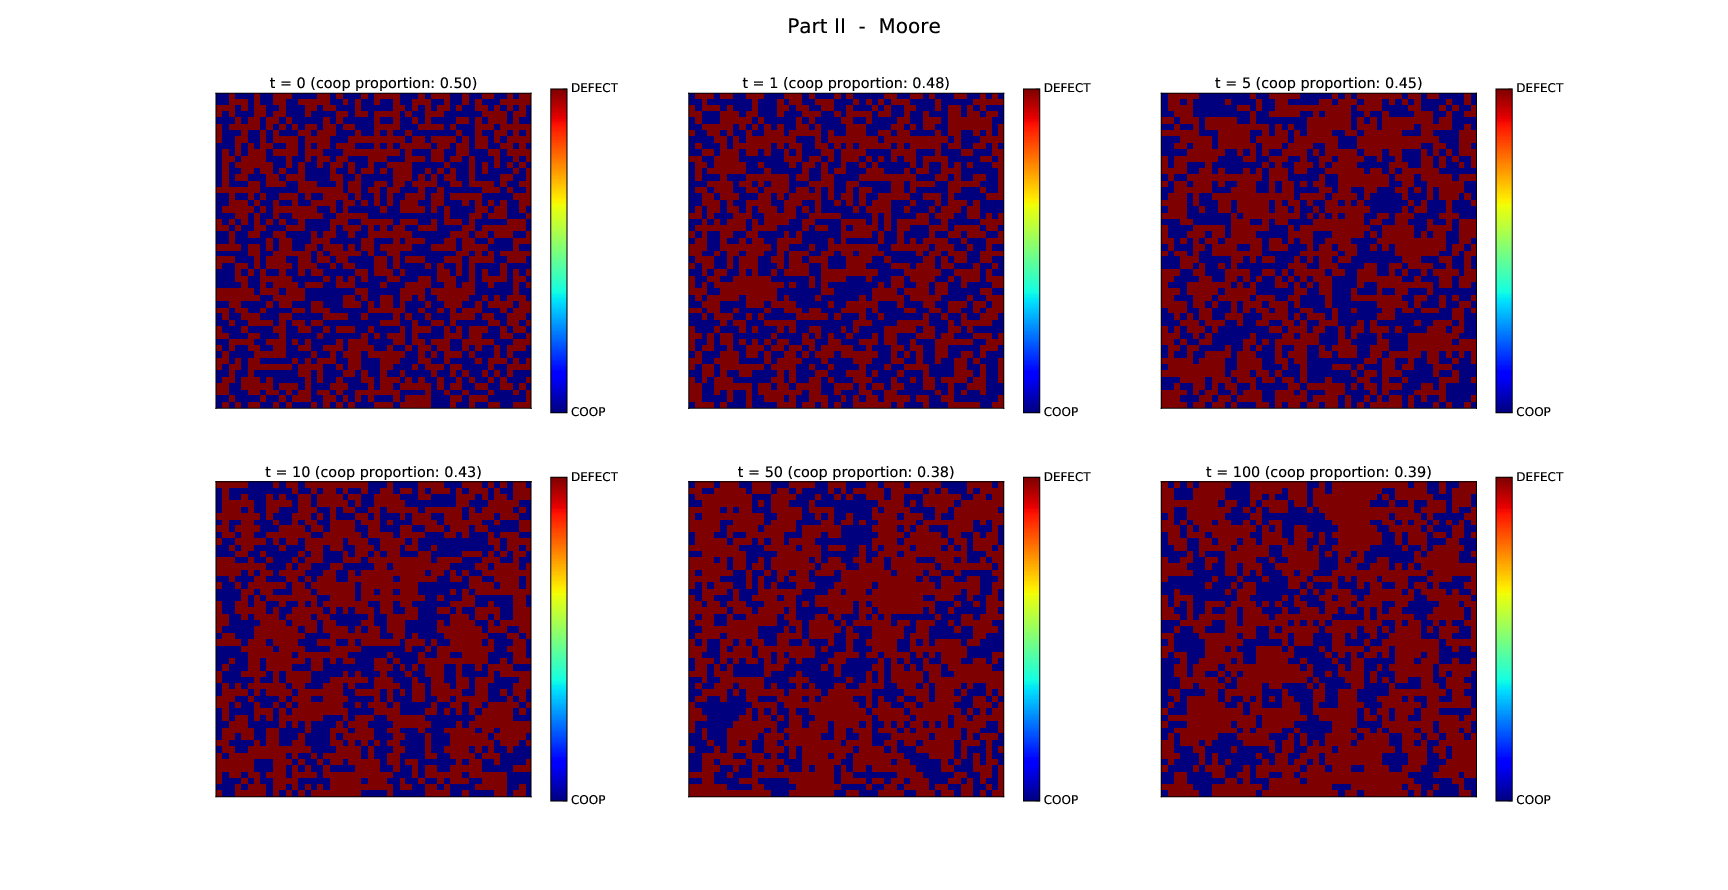
\includegraphics[width=1.2\textwidth]{imgs/part2_Moore_periods.png}
\caption{Spatial representation of a 50~x~50 lattice with agents playing Snowdrift Game at times $t=0,1,5,10,50,100$.
\label{fig:Spatial representation II.1}}
\end{figure}

\subsection{Von Neumann Neighbourhood Analysis}

\subsubsection{Cooperation Level}

This last study case is the only one for which the average cooperation level is not stabilized after $100$ steps:
we can see that as for the Moore Neighbourhood analysis of this second part, the curves are slowly decreasing
(faster in this case than in the previous one, but still way slower than the cooperation level drop that has
been observed in this first part), but don't reach a steady state. At time $t=100$, we see that the cooperation
level is around $20\%$, but seems to keep decreasing.

When looking at Figure~\ref{fig:replot of fig 1}, we see that the cooperation level converges to around $18\%$
for lattices with size $\geq$ 20~x~20 (the 12~x~12 is slightly below), the 4~x~4 lattice reaches convergence
around $6\%$, and the 8~x~8 keeps decreasing. Therefore, even though it takes more time, the cooperation level
reaches a steady state as well in this configuration.

\begin{figure}[!t]
\hspace{-1.8cm}
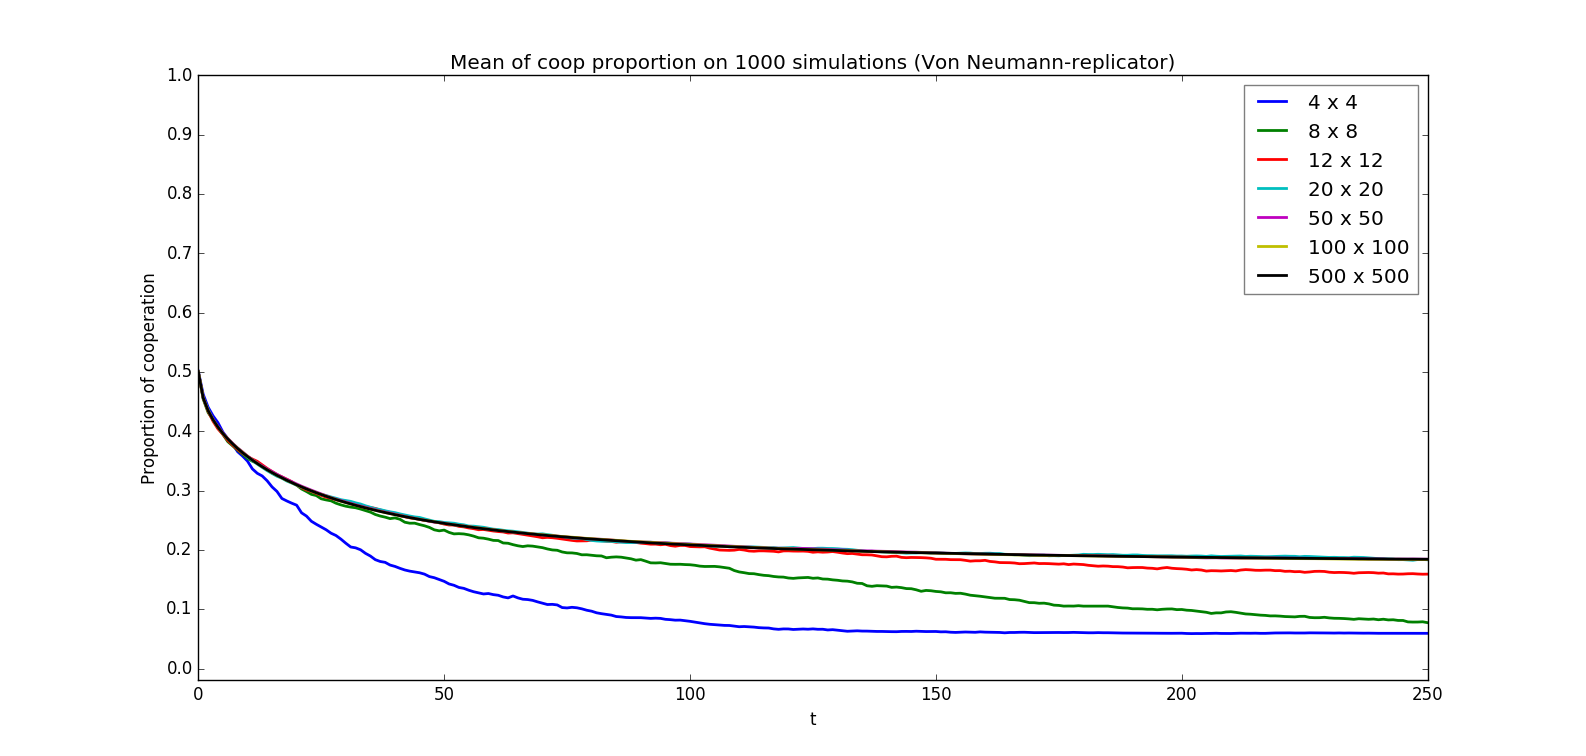
\includegraphics[width=1.2\textwidth]{imgs/fig_1_part_2_VN_0_to_250.png}
\caption{Average cooperation level of several square lattices (of dimension $n=4,8,12,20,50,100,500$) computed
on $10^4$ simulations for 250 steps.\label{fig:replot of fig 1}}
\end{figure}

Like in the Moore situation of this part, without considering the 4~x~4 and 8~x~8 lattices, the achieved
steady state does not depend on the lattice dimensions, and the discussion above still stands since it only
implies the replication rule, not the neighbourhood.

Yet, the reached steady state is lower than the previous one. This was expected since neighbourhood change
from Moore to Von Neumann brought a hard decrease in the cooperation level in first part; thus it is not
surprising that in this situation, the neighbourhood change also lead to a decrease. Note also that in first
part, this change of neighbourhood lead to a new steady state around $2.2$ times lower, and in this second
part, the division factor is again roughly $2.2$ ($\simeq 40/18$).

For completeness, Figures~\ref{fig:9a} and \ref{fig:9b} represent the distribution of payoffs and $p_{ij}$
probabilities in the 50~x~50 lattice with Von Neumann neighbourhood.

What can be observed is that at time $t=0$, the distinction between the two distribution is even more visible
than with the Moore neighbourhood: there seems to be an offset of around $20\%$ in the distributions (considering
that they are alike). Also, we can see that payoffs are really smaller, which is logical since the neighbourhood
size is divided by two, which implies that the maximum payoff is also divided by two.

Also, the $p_{ij}$ probability distribution has a higher variance and takes more possible values in this situation
than with a Moore neighbourhood.

\begin{figure}
	\begin{subfigure}{\textwidth}
		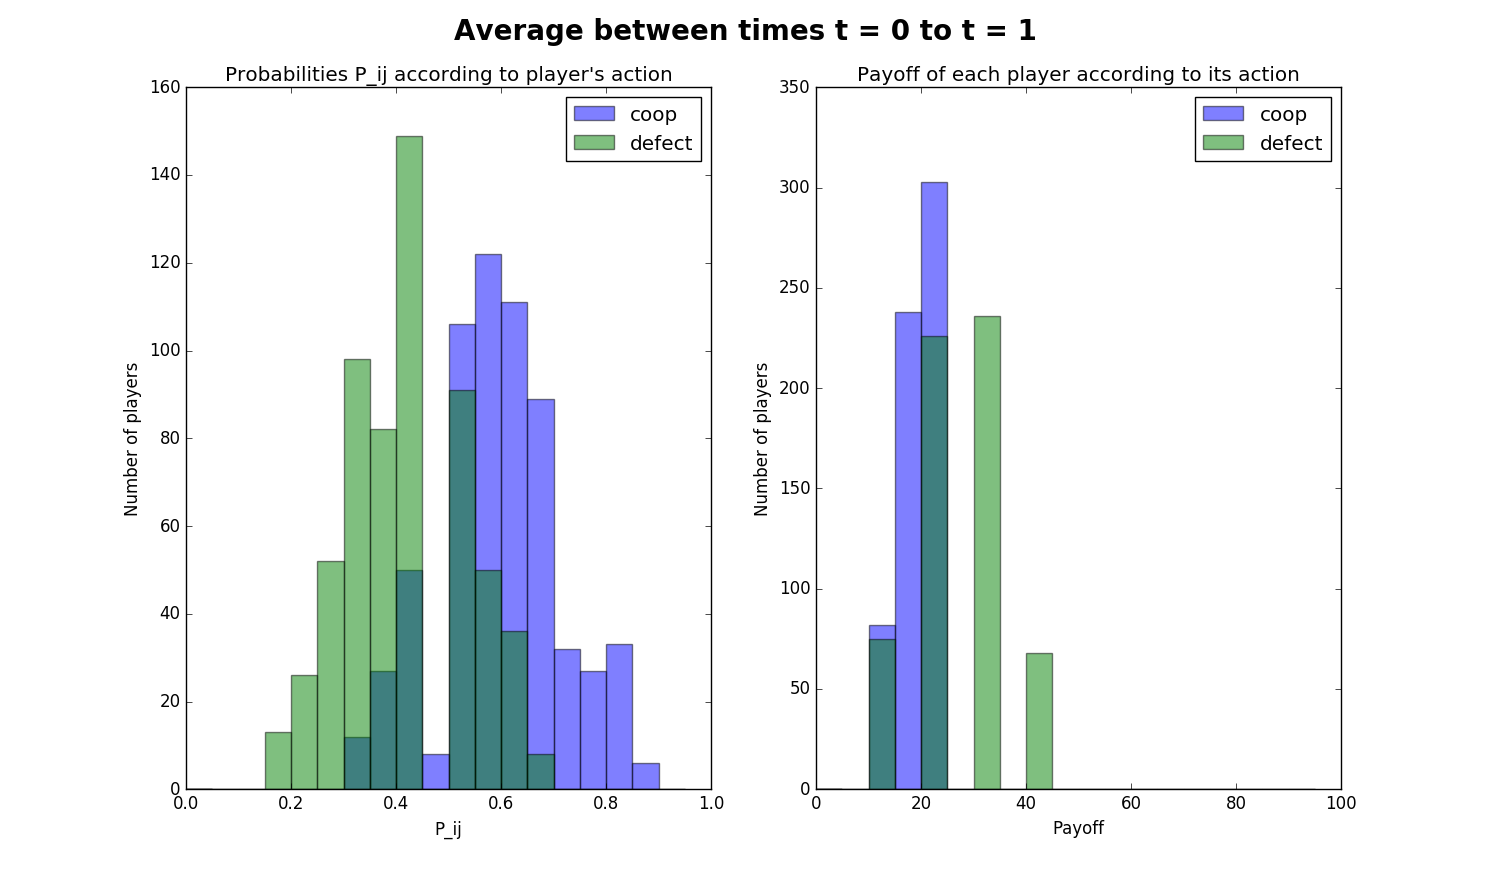
\includegraphics[width=\textwidth]{imgs/part2_diff_coop_defect_0_to_1_VN.png}
		\subcaption{Adaptation of Figure~\ref{fig:Part II hists coop/defect Moore 0 to 1} for Von Neumann
		Neighbourhood.\label{fig:9a}}
	\end{subfigure}
	\begin{subfigure}{\textwidth}
		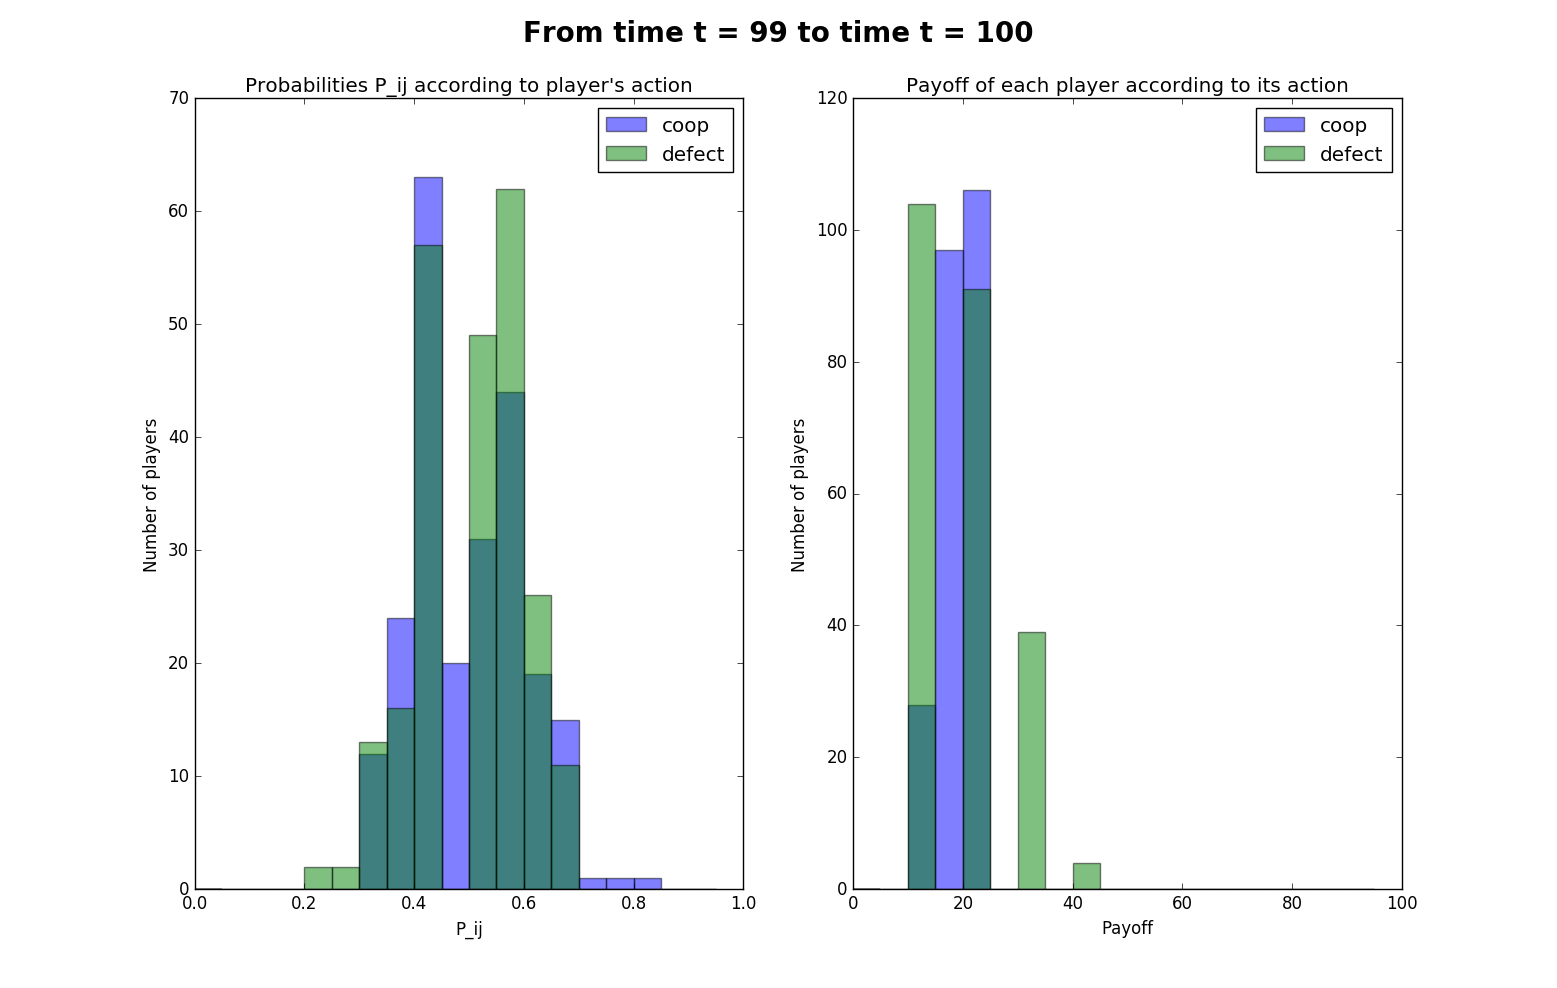
\includegraphics[width=\textwidth]{imgs/part2_diff_coop_defect_99_to_100_VN.png}
		\subcaption{Adaptation of Figure~\ref{fig:Part II hists coop/defect Moore 99 to 100} for Von Neumann
		Neighbourhood.\label{fig:9b}}
	\end{subfigure}
	\caption{Probability $p_{ij}$ and payoff of players in a 50~x~50 lattice when changing strategy.\label{fig:9}}
\end{figure}

The discussion about these distributions would be roughly identical to the one above, with the exception that
between times $t=99$ and $t=100$, is is hard to say that the difference between these distributions is negligible.
Yet, this is coherent with the cooperation level that is observed: the cooperation level on the lattice is
not stable at this time.

The $p_{ij}$ probability distribution and the payoff distribution of the 4~x~4 lattice are shown in
Figure~\ref{fig:hists coop/defect 4x4 VN} (by comparison with Figure~\ref{fig:Part II hists coop/defect Moore all 4x4}).
We see that the distribution is again broader, and that the distinction between probabilities to change from
cooperation to defection is on average bigger than the probability to change from defection to cooperation.

\begin{figure}[!t]
\hspace{-1.8cm}
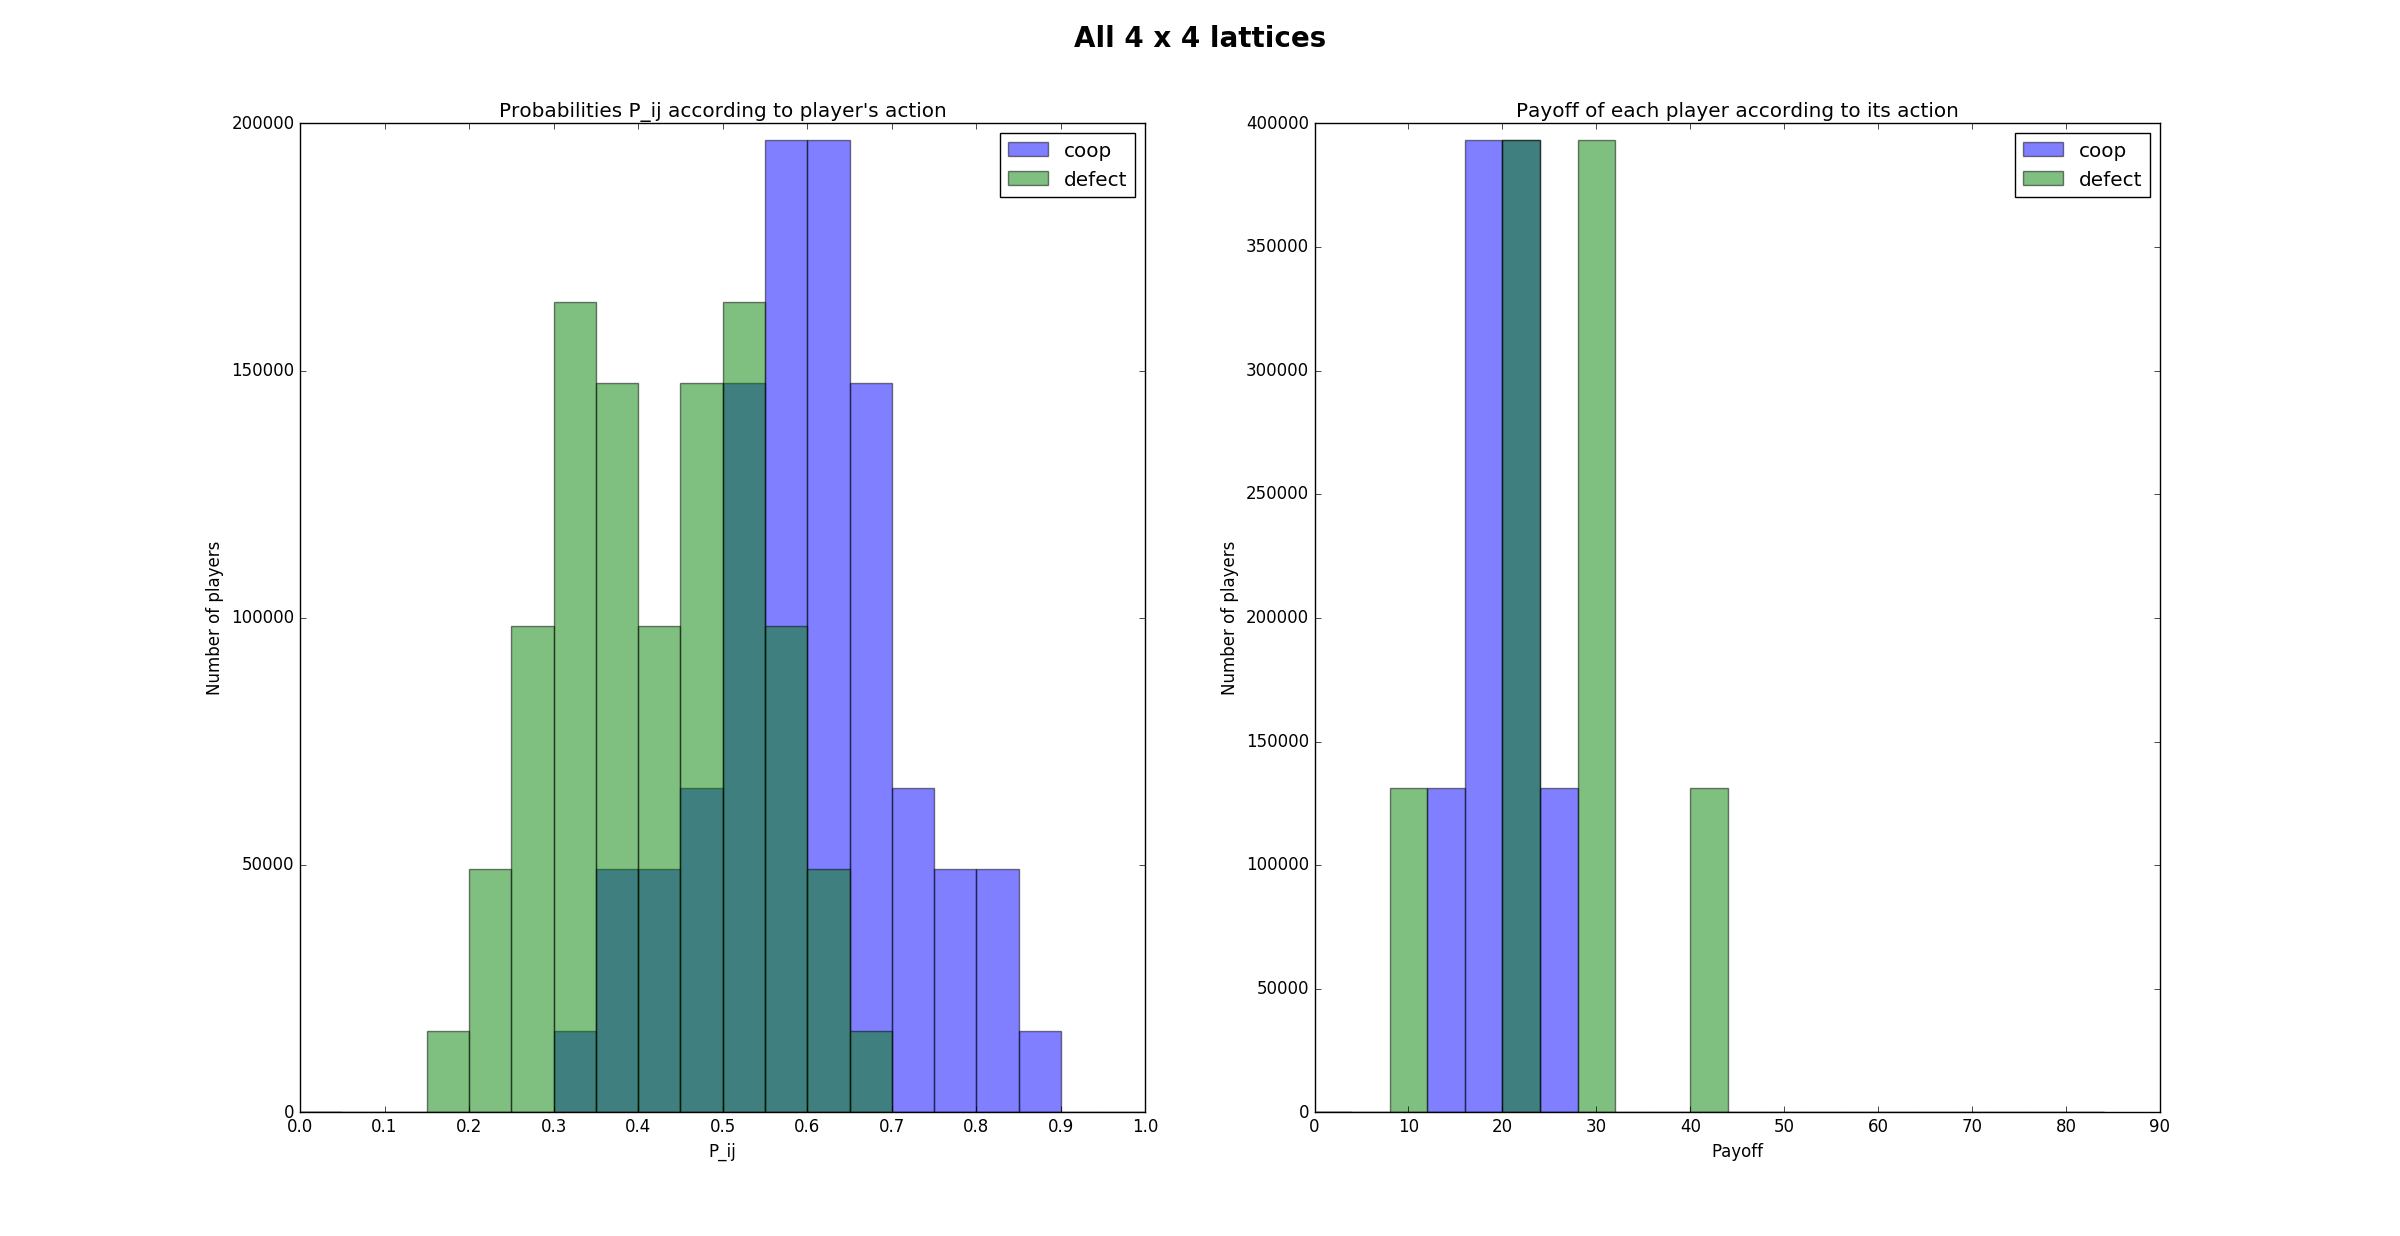
\includegraphics[width=1.2\textwidth]{imgs/part2_diff_coop_defect_0_to_1_4x4_VN.png}
\caption{Distribution of both $p_{ij}$ probability and payoff with a Von Neumann neighbourhood by taking all the
4~x~4 lattices into account.\label{fig:hists coop/defect 4x4 VN}}
\end{figure}

\newpage

\subsubsection{Spatial Representation}

On Figure~\ref{fig:spatial representation part II VN}, one can see the spatial representation of the lattice
with time. As discussed above, the replication rule used in this second part allows players to be surrounded
by only players with the opposite strategy (and to not change their own strategy). This can be observed in
all of the steps shown.

Note that for such \textit{lonely} players to be present in a quite large cluster, it is required that they
either have been stable there for several periods, or that they got \textit{stuck} in the merging of two
different clusters \textit{expanding}. These words written in italic are used because they are convenient
to describe what \textit{seems} to be happening, but keep in mind that each element of the lattice is considered
as a single agent that changes strategy with time, according to their neighbours' behaviour.

Also, in this situation, we can see that defecting players tend to form clusters, as opposed to the previous
case with Moore neighbourhood. Yet, even though some high density defection patterns tend to appear, they don't
come in a particular shape (such as rectangles as in first study case or diamonds as in second study case).

But as mentioned previously, the cooperation level stabilizes to a certain level (see previous subsubsection),
yet this doesn't mean that the lattice is static! It is quite remarkable when looking at times $t=50$ and $t=100$
(note that even if the cooperation level still hasn't stabilized at this point, it decreases sufficiently
slow to notice that consider it stabilized when looking at the \textit{movement} of the density).

\begin{figure}[!t]
\hspace{-1.8cm}
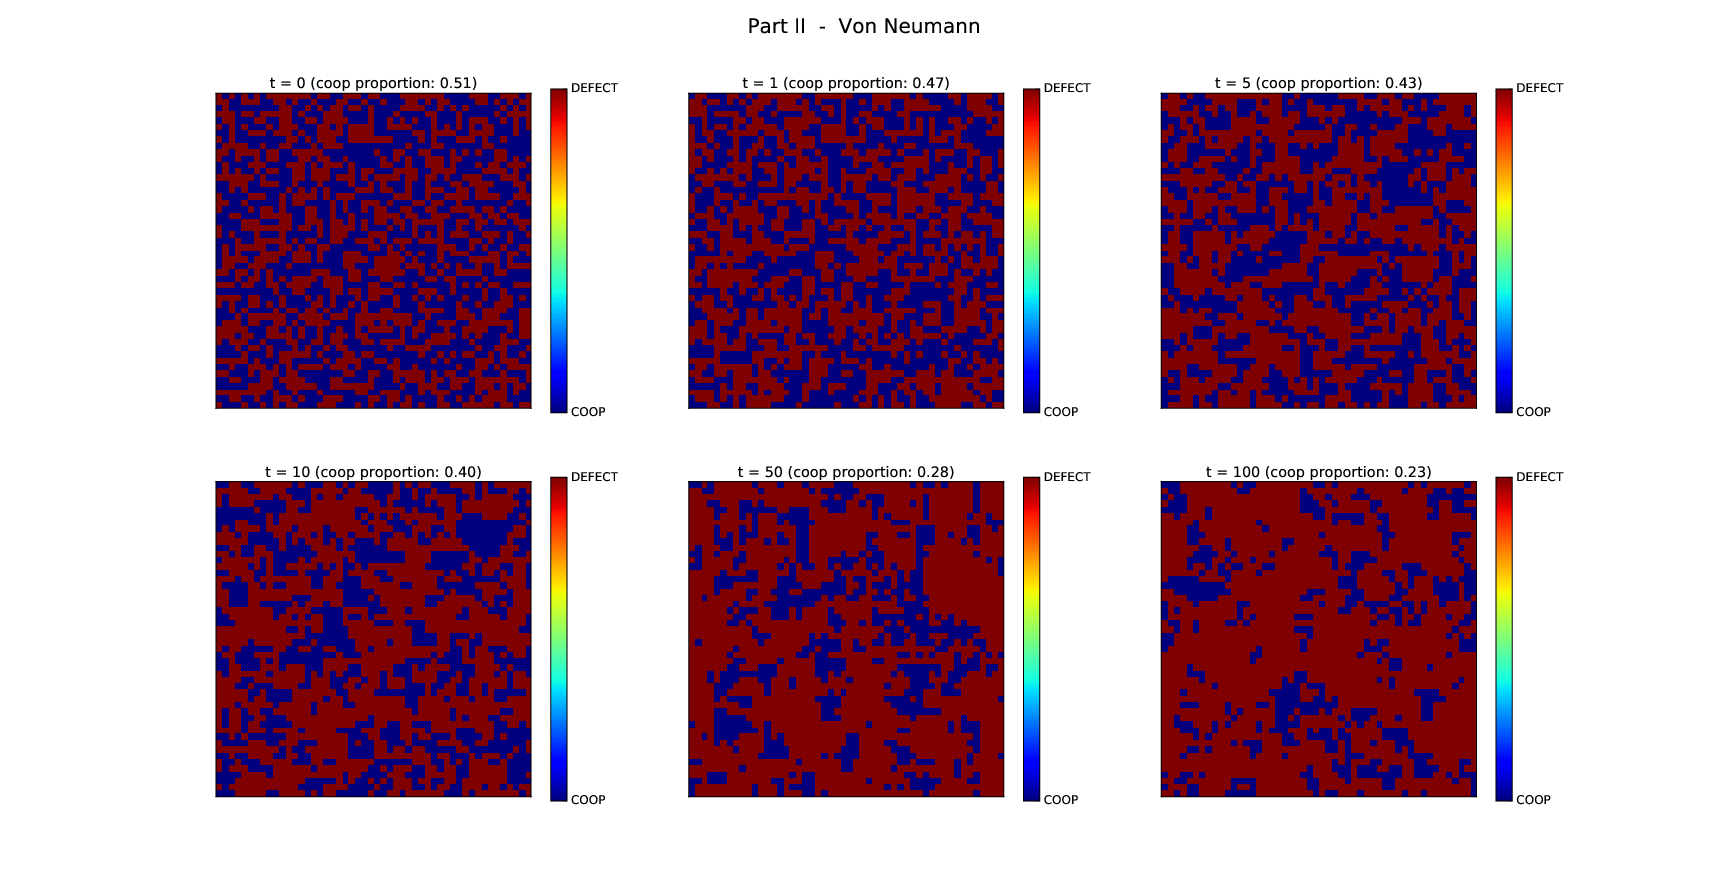
\includegraphics[width=1.2\textwidth]{imgs/part2_VN_periods.png}
\caption{Spatial representation of the 50~x~50 lattice playing Snowdrift with Von Neumann neighbourhood on
times $t=0,1,5,10,50,100$.\label{fig:spatial representation part II VN}}
\end{figure}

\section{Conclusion}

We have experimented on two types of neighbourhood in this document: Moore and Von Neumann neighbourhood,
both in two distinct situations: Prisoner Dilemma with Best neighbour replication rule, and Snowdrift with
stochastic replication rule.

For both these neighbourhood, the common observation was that a smaller neighbourhood lead to a smaller
average cooperation level on the lattice. Also, for Best Neighbour (first part), the change in neighbourhood
shape lead to a change in the cooperative clusters shape: from rectangles for Moore to diamonds for Von Neumann.

Also, when introducing stochastic behaviour (from first part to second part), the difference in cooperation level
related to the lattice size disappeared: no matter what is the dimension of the lattice, it converges to a given
steady state only depending on the neighbourhood (and the payoff matrix but which is not a changing factor in
this study).

With all of the differences that have been observed between each of these 4 study cases, we can say that both
these factors clearly change the behaviour of the lattice dynamics.

\end{document}
